\section{Wstęp}

\qquad Zespół QRS to fragment zapisu elektrokardiograficznego. Opisuje pobudzenie mięśni serca i składa się z jednego lub kilku załamków określanych jako Q, R i S.
\begin{itemize}
	\item Załamek R – każdy załamek dodatni w obrębie zespołu QRS
	\item Załamek Q – pierwszy ujemny załamek widoczny przed załamkiem R
	\item Załamek S – pierwszy ujemny załamek widoczny po załamku R
\end{itemize}
Przykładowy (wyidealizowany) zespół QRS widoczny jest na rys. \ref{fig:QRSComplex}, przedstawiającym schematyczny fragment zapisu elektrokardiograficznego.


\begin{figure}[h]
	\centering
	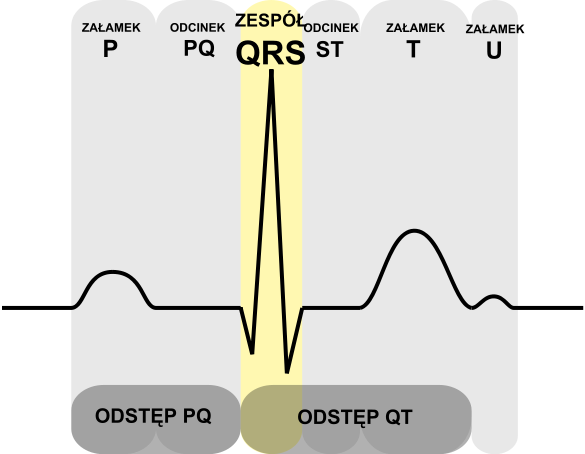
\includegraphics[width=0.8\textwidth]{Grafika/ZespolQRS}
	\caption{Wyidealizowany schemat zapisu EKG z zaznaczonym zespołem QRS. Źródło  \cite{QRSComplexWiki}}
	\label{fig:QRSComplex}
\end{figure}

\qquad Celem opisywanego modułu jest wyliczenie liczby klas zespołów QRS, określenie reprezentantów każdej z nich oraz oznaczenie klas zespołów QRS na wykresie ECG. Wyodrębnienie klas QRS występujących w sygnale ECG pozwala na określenie prawidłowości rytmu pracy serca. Z reguły nieregularności mają charakter przejściowy, dlatego ich poprawne wyznaczenie wymaga przeprowadzenia 24-godzinnego badania pracy serca, czyli testu Holtera \cite{RaportKoncowy}.